\chapter{Methodology}
\section{Initial Planning and Research}
\paragraph{When I first set out beginning this project I wanted to make sure I gave the planning phase enough attention. Often times in the past for previous college projects I found myself jumping straight into coding without having properly thought out and planned what I actually needed to do and in what order. This can often times lead to running into obstacles further down the line in the project that become harder and harder to revert or fix the longer they are left.}
\paragraph{I knew I wanted to use a JavaScript framework for the front end design. As I had initially planned on using the MEAN stack for the project I brought this up with my supervisor who informed me that this stack had been covered in some degree in the previous year, therefore it might seem as if I am not challenging myself enough with a new technology. Of course, I wasn't in this year and had no prior learning with it but opted to leave it nonetheless.}
\paragraph{After meeting my supervisor and swapping ideas I decided to do some further research into popular technologies for designing web applications and landed on React for the front end and MongoDB for the database tier. My supervisor recommended I look into Spring Boot or Dropwizard for the back-end side of things and from there I had a decent amount of material and technologies to familiarise myself with before the actual development of the application could begin.}
\paragraph{Although testing wasn't very high on my list, as is the case for many student projects, I knew I would need to at least 'dip my toe' into it. It was important for me to gain exposure to every facet of developing a full stack application. Research into testing React applications very quickly led me to 'Jest' and 'React Testing Library' which I will cover in further detail later.}

\section{Project Planning Tools and Project  Meetings}
\paragraph{As I did not form a group with any other students I simply set aside two hours every week for my own individual project meetings. I usually did this the day before meeting with my supervisor in order for things to be fresh in my mind with which to discuss. Of course as time goes on and depending on other project deadlines, I often went well over two hours a week and occasionally wen under this. I tried to always do something however. As I touched on before, I really didn't want to rush into coding before I had a decent idea of what I wanted to do and in what order I needed to do it. My supervisor was very helpful in this respect and used to set out weekly objectives for me to have completed before our next weekly meeting.}
\paragraph{As far as project planning tools, I initially used Trello. Trello is a project managing software that helps to visualise projects as well as organise workloads into different cards \cite{wiki:trello}. Initially, I used Trello quite a lot for planning and research as well as making sure I set objectives and deadlines for such research (Figure ~\ref{trello_label}). As the weeks went on however I found myself using it less and less and instead, just noting what goals I wanted to achieve in a diary instead.}
\begin{figure}
        \centering
        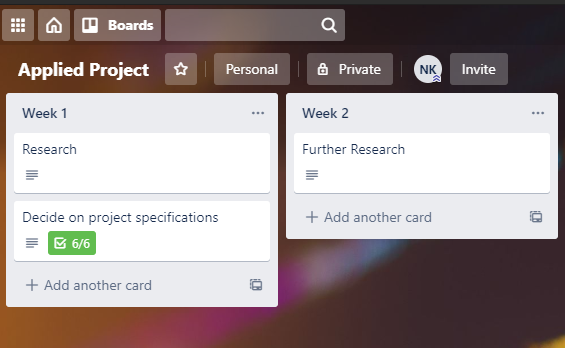
\includegraphics[scale=0.6]{Images/Trello.png} 
        \label{trello_label}
        \caption{My Trello Board}
\end{figure}

\section{Github as a Development Tool}
\paragraph{As with all projects I undertake, I used Git for version controlling the application as well as backing up the application. Looking back, I feel I didn't utilise Github as well as I would have liked. Github offers a lot of functionality such as the issue tracker or the wiki. I largely only used Git for backing up my project and always having the source code accessible from any device.}
\paragraph{If I was to start the development of this project again I would definitely have used the issue tracker as often as possible to show the problems I faced with development as well as how I overcame them. I began using the issue tracker very late in the project and I only managed a small handful of entries.Not using it throughout is a  big regret I have, since I 've started using it I've found it's a great way to showcase your thinking at each stage of a problem. I also would've used branches to always keep a clean working copy of my application available that I could revert to at any time. Git is a very important tool to software development and I feel I might have used this opportunity better to showcase my understanding of it more.}
\paragraph{The wiki is another powerful feature I might have used. The wiki provide a place in your repository to lay out the road-map of your project, show the current status, and document software better. I instead opted to simply keep a Word diary on my local machine, that I made entries to whenever I worked on the project. I believe documenting your thinking during development is very important.}
